Before the comparison with the state of the art distributed algorithms in Section~\ref{Experiments}, we performed a set of experiments to measure the performance impact of the maximum expansion threshold, evaluating the quality of a set of proposed strategies. This set of experiments, together with the ones in Section~\ref{Experiments}, are performed on two real life datasets.
The first real dataset is the \textbf{Kent Ridge Breast Cancer}~\cite{breast_cancer_dataset}, which contains gene expression data.
It is characterized by 97 rows that represent patient samples, and
24,482 attributes related to genes. The attributes are numeric (integers, floating point).
Data have been discretized with an equal depth partitioning
using 20 buckets (similarly to \cite{Zaki_Carpenter}).
The second real dataset is the \textbf{PEMS-SF} dataset~\cite{breast_cancer_dataset}, 
which describes the occupancy rate of different car lanes of San Francisco bay area freeways.
Each transaction represents the daily traffic rate of 963 lanes, sampled every 10 minutes.
It is characterized of 440 rows (in some experiments we have utilized only the first 100) and 138672 attributes (6 x 24 x 963), and it has been discretized in
equi-width bins of 0.002.
Because of their distribution and their discretizazion process, the Breast Cancer dataset is more sparse (low correlation among the dataset transactions) than the PEMS-SF dataset. 
The other two datasets were synthetically generated and tuned to simulate
use cases characterized by extremely high-dimensional data,
i.e., with massive numbers of features.
Both datasets consists of 30 transactions.
Dataset~\#1 has 1,000,000 different items
and an average transaction length of 500,000 items,
while
Dataset~\#2 is 10 times larger, with 10,000,000 different items
and an average transaction length of 5,000,000 items
(see Table~\ref{datasets}).
The discretized version of the real dataset and the synthetic dataset generator
are publicly available at http://dbdmg.polito.it/PaMPa-HD/. \textbf{TO DO: aggiungere versione finale discretized pemsf}



\begin{table}[h!]
\begin{center}
\caption{Datasets}
\label{datasets}
\begin{tabular}{|c|c|c|c|}
\hline
	Dataset & Number of  & Number of & Average number  \\
	 & transactions &different items & of items  \\ 
	  &  & &  per trasanaction  \\ \hline
	Kent Ridge Breast    & 97 & 489,640    & 24,492 \\
     CancerDataset      &    &            &  \\ \hline
PEMS-SF    & 440& 5,454,414     & 138,672 \\
     Dataset      & (100 rows version)   &   (3,946,646)       &  \\ \hline
	Synthetic Dataset \#1 & 30 & 1,000,000  & 500,000\\ \hline
	Synthetic Dataset \#2 & 30 & 10,000,000 & 5,000,000\\ \hline
\end{tabular}
\end{center}
\end{table}


PaMPa-HD is implemented in Java 1.7.0\_60 using the Hadoop MR API.
Experiments were performed on a cluster of 5 nodes running Cloudera
Distribution of Apache Hadoop (CDH5.3.1).
Each cluster node is a 2.67 GHz six-core Intel(R) Xeon(R) X5650 machine
with 32 Gbyte of main memory
running Ubuntu 12.04 server with the 3.5.0-23-generic kernel.


\subsection{Impact of the maximum expansion threshold}\label{exp_fisso}
As already mentioned in Section~\ref{Distributed implementation outline}, the maximum expansion threshold
($max\_exp$) parameter indicates the maximum number of nodes 
to be explored before a preemptive stop of each distributed sub-process is forced.
This parameter strongly affects the enumeration tree exploration,
forcing each parallel task to stop before completing the visit of its sub-tree 
and write partial results on HDFS. 
This approach allows the synchronization job to globally apply 
pruning rule 3 and reduce the search space.
Low values of $max\_exp$ threshold decrease the risks of memory issue, 
because the global problem is split into simpler and less memory-demanding
sub-problems, and facilitate the application of pruning rule 3, 
hence a smaller subspace is searched.
However, higher values allow a more efficient execution,
by limiting the start and stop of distributed tasks
(similarly to the context switch penalty), and the synchronization overheads.

In order to assess the impact of the expansion threshold parameter, we performed two set of experiments. In the first one we have performed the mining on the PEMS-SF (100 transactions) dataset with a Minsup 50, by varying $max\_exp$ from 10 to 100,000,000.  The minsup value was empirically selected in order to let the mining problem being deep enough to show up different performances. 
In Figure~\ref{pems_fixed} are shown the results in terms of execution time and number of iterations 
(i.e., the number of jobs).

It is clear how the $max\_exp$ parameter can influence the performance, with wall-clock times that can be doubled with different configurations. The best performance in terms of execution time is achieved with a maximum
expansion threshold equal to 10,000 nodes. With lower values, the execution times are slightly longer, while there is an evident performance degradation with higher $max\_exp$ values. 
This result highlights the importance of the synchronization phase.
Increasing the $max\_exp$ parameter makes the number of iterations decreasing,
but more useless tree branches are explored,
because pruning rule 3 is globally applied less frequently.
Lower values of  $max\_exp$, instead, raising the number of iterations
, introduce a slight performance
degradation caused by iterations overheads.
%With very high values of  $max\_exp$, the running time and the number of
%iterations are stable because the bottleneck becomes the free available
%memory, and the synchronization job is
%automatically applied, independently of the value of  $max\_exp$.

\begin{figure}[!t]
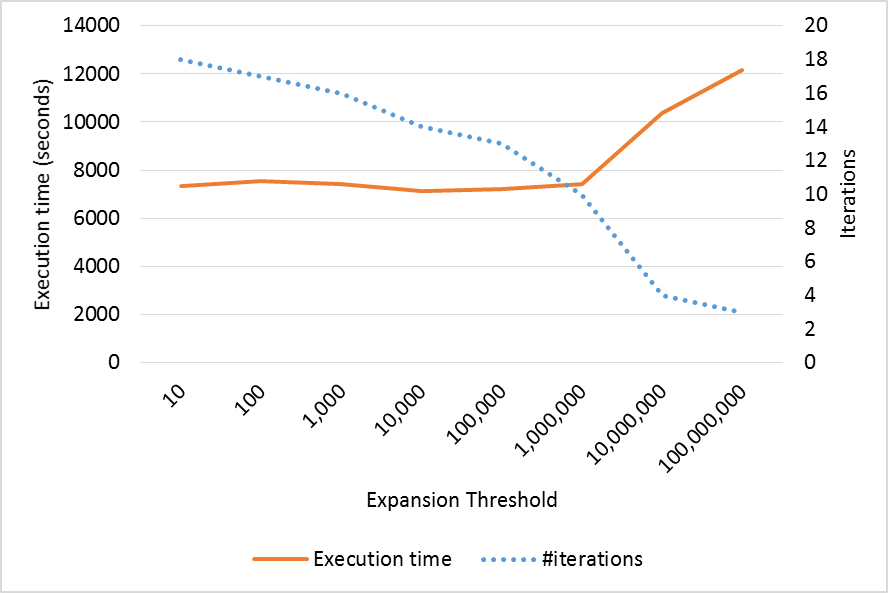
\includegraphics[width=5in]{immagini_extension/pems_fixed.png}
\caption{Execution time and number of iterations for different $max\_exp$ values on PEMS-SF dataset with $minsup$=50.
}
\label{breast_fixed}
\end{figure}

\begin{figure}[!t]
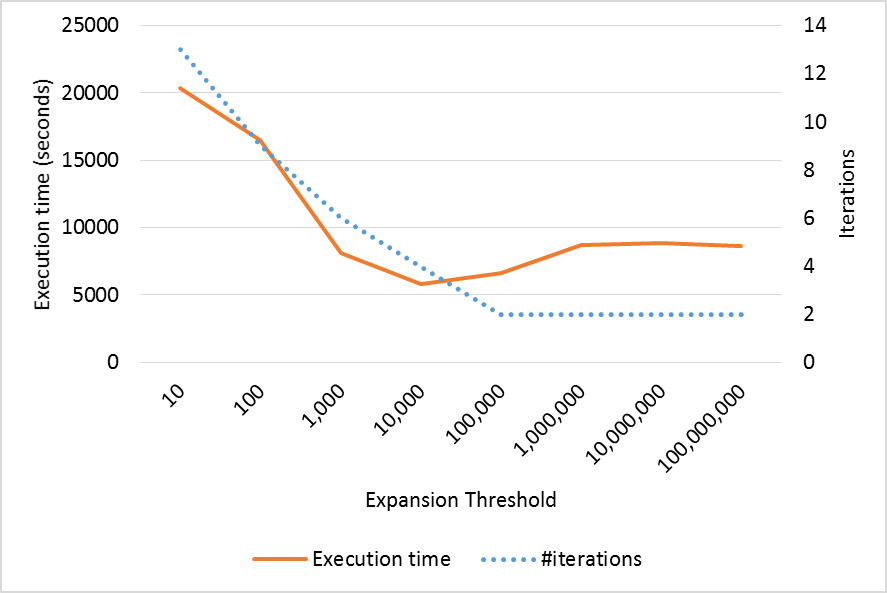
\includegraphics[width=5in]{immagini_extension/breast_fixed.png}
\caption{Execution time and number of iterations for different $max\_exp$ values on Breast Cancer dataset with $minsup$=6.
}
\label{pems_fixed}
\end{figure}

The same experiment is repeated with the Breast Cancer dataset and a minsup value of 6. As shown in Figure~\ref{breast_fixed}, this time the best performances are achieved with $max\_exp$ equal to 100,000. In this case, indeed, cannot be noted big differences with the higher values. Instead, the performances strongly decreases with lower values of $max\_exp$ parameter.



\textbf{+ menzione a load balancing}.







The $max\_exp$ choice has a non-negligible impact on the performances of the algorithm. As demonstrated by the curves in Figures~\ref{pems_fixed} and~\ref{breast_fixed}, it is very dependent on the use case and distribution of the data. In order to simplify the parameter configuration for the user and, above all, increase the performance of the algorithm, we have implemented some tuning strategies related to $max\_exp$, prensented in the next subsection.
%
%This set of experiments has been performed on the Breast cancer dataset
%with Minsup 5, by varying $max\_exp$ from 100 to 100,000,000. This minsup value allowed to notice different
%wall-clock time for each expansion threshold value.
%Figure~\ref{exp_1} shows the results in terms of execution time and number of iterations 
%(i.e., the number of jobs).
%The best performance in terms of execution time is achieved with a maximum
%expansion threshold equal to 10,000 nodes.
%With higher values, the number of iterations decreases,
%but more useless tree branches are explored,
%because pruning rule 3 is globally applied less frequently.
%Lower values of  $max\_exp$, instead, introduce a performance
%degradation caused by the higher number of iterations
%and the synchronization phase overheads.
%With very high values of  $max\_exp$, the running time and the number of
%iterations are stable because the bottleneck becomes the free available
%memory, and the synchronization job is
%automatically applied, independently of the value of  $max\_exp$.
%The tuning of $max\_exp$ is strictly related to the data distribution:
%in general, the easier the mining task, the fewer the benefits of having 
%many iterations.
%
%The value of $max\_exp$ impacts also the load balancing 
%of the distributed computation among different nodes.
%With low values of $max\_exp$, each task explores a
%smaller enumeration sub-tree, decreasing the size difference
%among the sub-trees analyzed by different tasks,
%thus improving the load balancing.
%Table~\ref{load balance} reports the minimum and the maximum execution time of
%the mining tasks executed in parallel for two extreme values of $max\_exp$. 
%The load balance is better for the lowest value of $max\_exp$.
%\textbf{tutto vecchio fin qui}
%
%
%\begin{figure}[!t]
%\includegraphics[width=3.5in]{grafo_exp2.png}
%\caption{Execution time and number of iterations for different $max\_exp$ values on Breast Cancer dataset with $minsup$=5.
%}
%\label{exp_1}
%\end{figure}
%
%
%\begin{table}
%\begin{center}
%\caption{Load Balancing}
%\label{load balance}
%\begin{tabular}{ |c| c | c| }
%\hline
%							    &
%\multicolumn{2}{|c|}{Task execution time}          \\ \hline
%	Maximum expansion threshold &   Min          & Max            \\ \hline
%	100,000,000                 &    4s                      & 1h 54m 33s
%  \\ \hline
%100,000                 &    4s                      & 1h 2m 32s
%  \\ \hline
%	10000                         &    4s                      &        23m 50s
%\\ \hline
%100                         &    4s                      &        53s
% \\ \hline
%\end{tabular}
%\end{center}
%\end{table}


\subsection{Proposed strategies}\label{exp_strategies}
This section introduces some heuristic strategies related to the $max\_exp$ parameter. 
The aim of this experiment is to identify an heuristic technique which is able to deliver good performances without the need by the user to tune up the the $max\_exp$ parameter.
Before the introduction of the techniques, let us motivate the reasons behind their design.
Because of the enumeration tree architecture, the first tables of the tree are the most populated. Each node, in fact, is generated from its parent node as a projection of the parent transposed table on a tid. 
In addition, the first nodes are, in the average, the ones generating more sub-branches. By construction, their transposed table tidlists are, by definition, longer than the ones of their children nodes. This increases the probability that the table could be projected on a tid.
For these reasons, the tables of the initial mining phase are the most heavy to be processed.
On the other hand, the number of nodes to process by each local Carpenter iteration tends to increase with the number of iterations. Still, this factor is mitigated by (i) the decreasing size of the tables and (ii) the eventual end of some branches expansion (i.e. when there are not more tids in the node transposed table).
These reasons, motivated us to introduce some strategies that assumes a maximum expansion threshold that is increased with the number of iterations. These strategy start with very low values in very initial iterations  (i.e. when the nodes are more heavy to be processed) and increase $max\_exp$ during the mining phases.

%Finally, in all the experiments \textbf{citare quelli di prima}, we have notices some very short execution times (less than a minute) in the last mining iterations. This surely increases the impact of MapReduce job handling overhead on the global performances.
%All these things, motivated us to introduce some strategies that assumes a maximum expansion threshold that is increased with the number of iterations.
%All these things, together with very short last iterations (with an increasing MapReduce job overhead), motivated us to test some strategies that assumes a maximum expansion threshold that is increased with the iterations.

The strategy \#1 is straightforward: the $max\_exp$ is increased with a factor of $X$ at each iteration. For instance, if the $max\_exp$ is set to 10, and $X$ is set to 100 at the second iteration it is raised to 1000 and so on. 

Alternatively, we wanted to achieve a balanced growth of the $max\_exp$ parameter. We want to balance the load of the iterations, but, on the other hand, we want to avoid an overgrowth of the parameter and, therefore, of the execution times of the last iterations. As already said, in fact, increasing the $max\_exp$ parameter decreases the impact of the synchronization job pruning.
In order to monintor the growth, we introduced a set of techniques based on the execution times and a strategy which monitors the impact of the synchronization jobs.
%In order to monitor this growth, we firstly thought about an index measuring the effectiveness of the pruning in terms of closed or tables pruned in the synchronization job. However, the effectiveness of the pruning cannot be easily interpreted. An increasing pruning effect means that there are a lot of tables that are generated uselessly. However, an increasing pruning effect is also normal since the number of nodes that are processed continues to increase. \textbf{inserire degli esperimenti in cui faccio vedere che usare il pruning effect riduce le performance}.
In strategies \#2 and \#3, we took into exam the execution time of the iterations.
Spefically, strategy \#2 consists in increasing, at each iteration, the $max\_exp$ parameter with a factor of  $X^{T_{old} / T_{new}}$, given $T_{new}$ and  $T_{old}$ the execution time of the previous two jobs. The motivation is to balance the growth of the parameter in order to achieve a stable execution times among the iterations.  
Strategy \#3, instead, is inspired by the congestion control of TCP/IP (a data transmission protocol used by many Internet applications \cite{}). Precisely, the $max\_exp$ is handled like the congestion window size (i.e. the number of packets that are sent without congestion issues).
This strategy, called ``Slow Start'', assumes two types of growing of the window size: an exponential one and a linear one. In the first phase, the window size is increased exponentially until it reaches a threshold (``ssthresh'', which is calculated empirically from RTT and other values). From that moment, the growth of the window becomes linear, until a data loss occurs.
In our case, we are not interested we just inherit the two growth factors. Therefore, our ``slow start'' strategy consists in increasing the $max\_exp$ of a factor of $X$ until the last iteration reaches an execution time greater than a given threshold. After that, the growth is more stable, increasing the parameter of a factor of 10 (for this reason $X$>10).
We have fixed the threshold to the execution time of the first two jobs (Job 1 and Job 2). These jobs, for the architecture of our algorithm, consists of the very first Carpenter iteration. They are quite different than the others since the first Mapper phase has to build the initial projected transposed tables (first level of the tree) from the input file. 
We have selected the execution time of the first iteration since it is consistent with our initial aim,
that is to normalize the execution times of the last iterations which are often shorter than the first ones.

The last strategy, \#4, is based on the effectiveness of the pruning in terms of closed or tables pruned in the synchronization job. Indeed, the measure of the relative number of tables that are pruned cannot be easily interpreted. An increasing pruning percentage means that there are a lot of tables that are generated uselessly. However, an increasing trend is also normal, since the number of nodes that are processed continues to increases. Given that our intuition is to rise the  $max\_exp$ among the iterations, in strategy \#4, we increase the $max\_exp$ parameter with a factor $X^{Pr_{old} / Pr_{new}}$, given $Pr_{new}$ and  $Pr_{old}$ the relative number of pruned tables in the previous two jobs. 
%Even if strategy \#4 can be meant as the dual of strategy \#2, with the usage of the pruning ratios instead of the different execution times, we decided not to do the same for strategy \#3. In this case, we could not identify a proper threshold to be used for changing the growth factor of $max\_exp$. In strategy \#3, we have used the first iteration because the initial motivation of this empirical study is to stabilize the execution times. In this case, we don't consider the initial pruning ratio as a valid threshold: it is computed after only few tables and, in the worst case, can be 0.

In our experiment, we have fixed the initial  $max\_exp$ value to 10. This very low value is motivated by the nature of our strategies, which consist of a balanced increasing of the parameter.
We applied the strategies (resumed in Table~\ref{table_strategies}) to the same experiments of Figures~\ref{breast_fixed} and ~\ref{pems_fixed}, in order to compare execution times the ones obtained with the optimum choice of $max\_exp$. 
In oder to assess the impact of the $X$ parameter, we have used values from 10 to 10,000 (except for strategy3 for which we have used values from 100 to 10,000).

The result of the application of the techniques to the PEMS-SF dataset are shown in Figures~\ref{pems_strategy1},~\ref{pems_strategy2},~\ref{pems_strategy3},~\ref{pems_strategy4}, which represent the relative execution time gain with respect to the best execution time obtained with the fixed $max\_exp$ of 10,000. In Figure~\ref{pems_strategy_best} we have grouped the best configuration for each strategy in order to easily compare them.
It is clear how the almost all the strategies improve the performance of the algorithm. Only Strategy3 showed to be slower. Strategy1(1,000), Strategy2(10,000) and Strategy4(1,000) achieve a very similar speedup. 

We have repeated the experiment with Breast Cancer dataset and a minsup value of 6 (Figures~\ref{breast_strategy1},~\ref{breast_strategy2},~\ref{breast_strategy3},~\ref{breast_strategy4}). We have raised $X$ from 10 to 10,000. Only with Strategy2, as shown in Figure~\ref{breast_strategy2}, we have raised it to 100,000 , because the experiments could suggest a decreasing execution times trend, but it was not the case.
As before, the results are grouped in Figure~\ref{breast_strategy_best}.
In this case, all the strategies achieve a positive speedup with respect to the best execution time obtained with a fixed $max\_exp$ parameter. In addition, the same configurations for each strategy demonstrated to be most performant in both the experiments.
The results obtained with the adoption of these strategies are very similar, and the differences are negligible.



\begin{table}
\begin{center}
\caption{Strategies}
\label{table_strategies}
\begin{tabular}{|c|c|}
\hline
Strategy \#1($X$)  & Increasing at each iteration      \\ 
                   & with a factor of $X$               \\ \hline

Strategy \#2($X$)  & Increasing at each iteration with \\
                   & a factor of $X^{T_{old} / T_{new}}$                   \\ \hline

Strategy \#3       & Slow start, with a fast increase                      \\ 
     & factor of   $X$                     \\ \hline
Strategy \#4($X$) & Increasing at each iteration with \\
                   & a factor of $X^{Pr_{old} / Pr_{new}}$                    \\ \hline
            
\end{tabular}
\end{center}
\end{table}

\begin{figure}[!t]
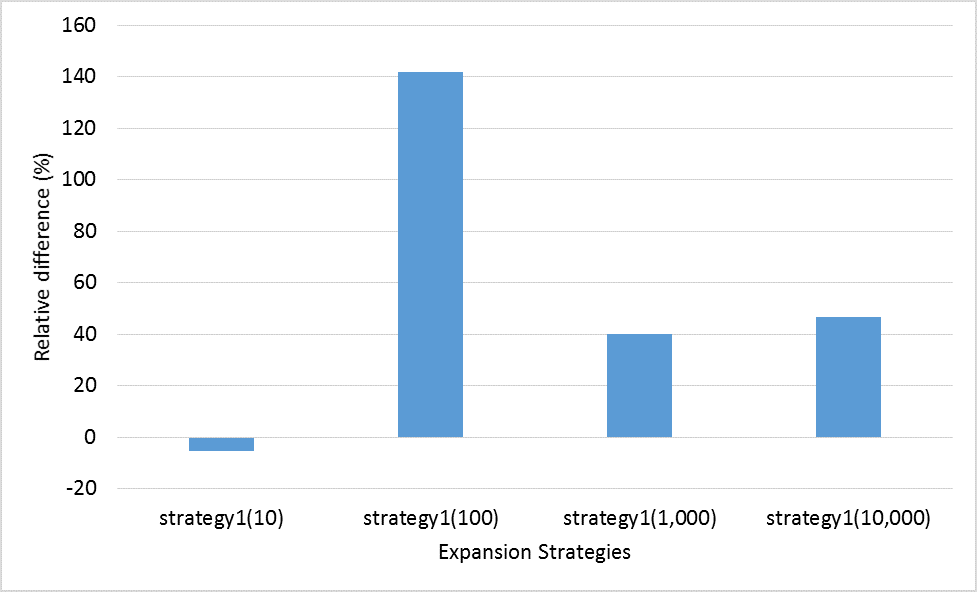
\includegraphics[width=5in]{immagini_extension/pems_strategy1.png}
\caption{Relative gains on Pems-SF dataset with $minsup$=50, Strategy1 and different $X$ values.
}
\label{pems_strategy1}
\end{figure}

\begin{figure}[!t]
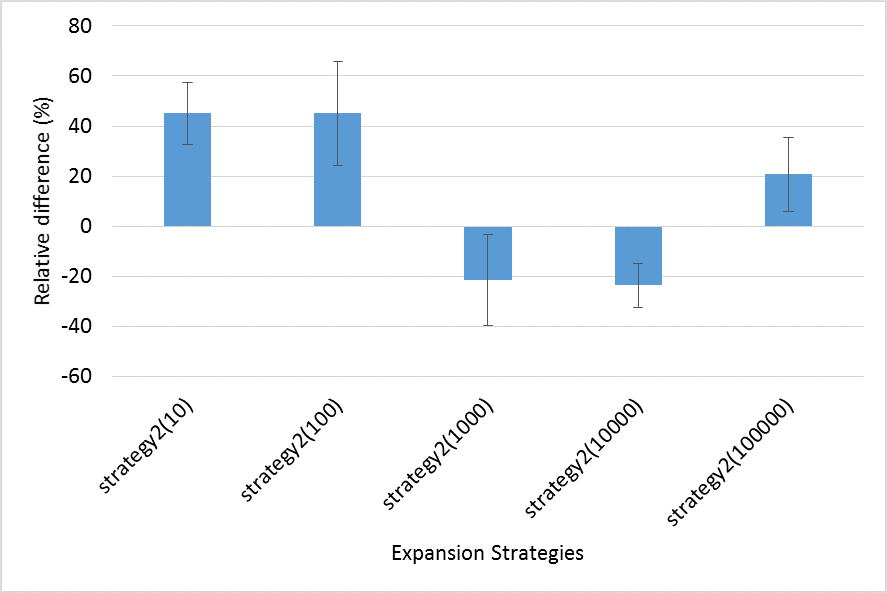
\includegraphics[width=5in]{immagini_extension/pems_strategy2.png}
\caption{Relative gains on Pems-SF dataset with $minsup$=50, Strategy2 and different $X$ values.
}
\label{pems_strategy2}
\end{figure}

\begin{figure}[!t]
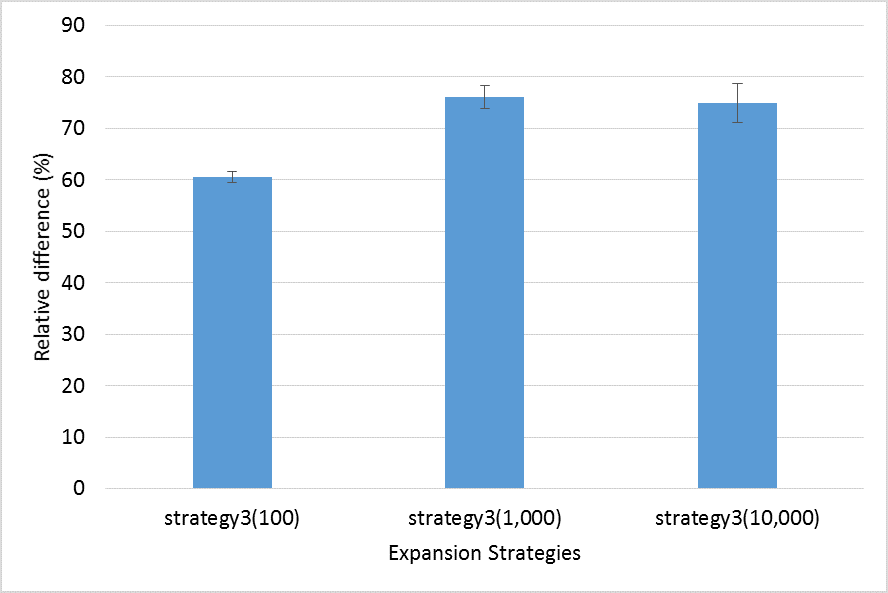
\includegraphics[width=5in]{immagini_extension/pems_strategy3.png}
\caption{Relative gains on Pems-SF dataset with $minsup$=50, Strategy3 and different $X$ values.
}
\label{pems_strategy3}
\end{figure}

\begin{figure}[!t]
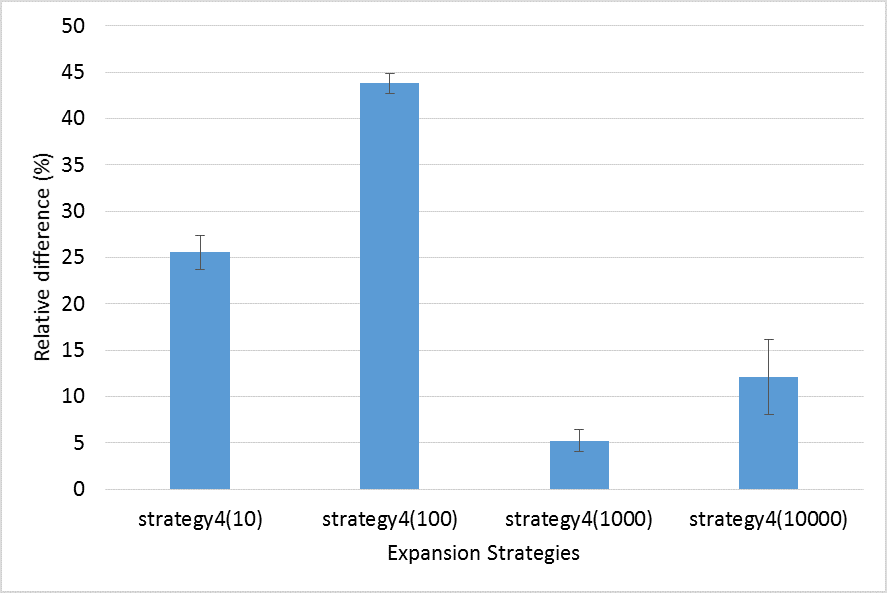
\includegraphics[width=5in]{immagini_extension/pems_strategy4.png}
\caption{Relative gains on Pems-SF dataset with $minsup$=50, Strategy4 and different $X$ values.
}
\label{pems_strategy4}
\end{figure}

\begin{figure}[!t]
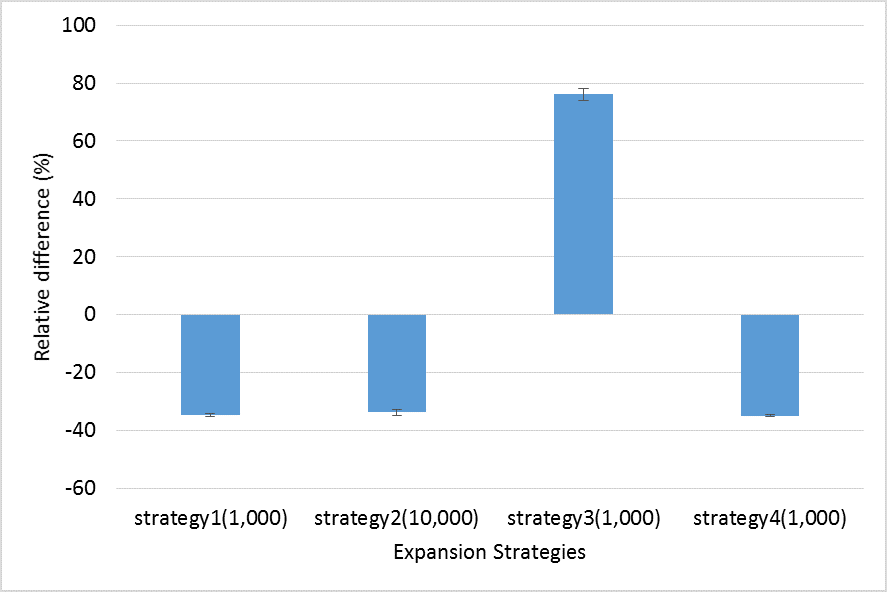
\includegraphics[width=5in]{immagini_extension/pems_strategy_best.png}
\caption{Relative gains of the best configuration for each strategy, on Pems-SF dataset with $minsup$=50.
}
\label{pems_strategy_best}
\end{figure}


\begin{figure}[!t]
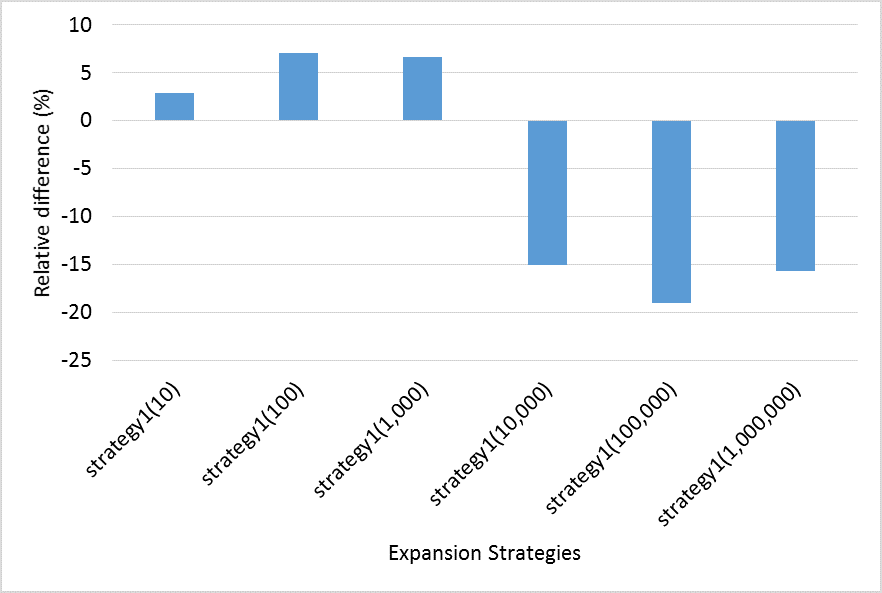
\includegraphics[width=5in]{immagini_extension/breast_strategy1.png}
\caption{Relative gains on Breast dataset with $minsup$=6, Strategy1 and different $X$ values.
}
\label{breast_strategy1}
\end{figure}

\begin{figure}[!t]
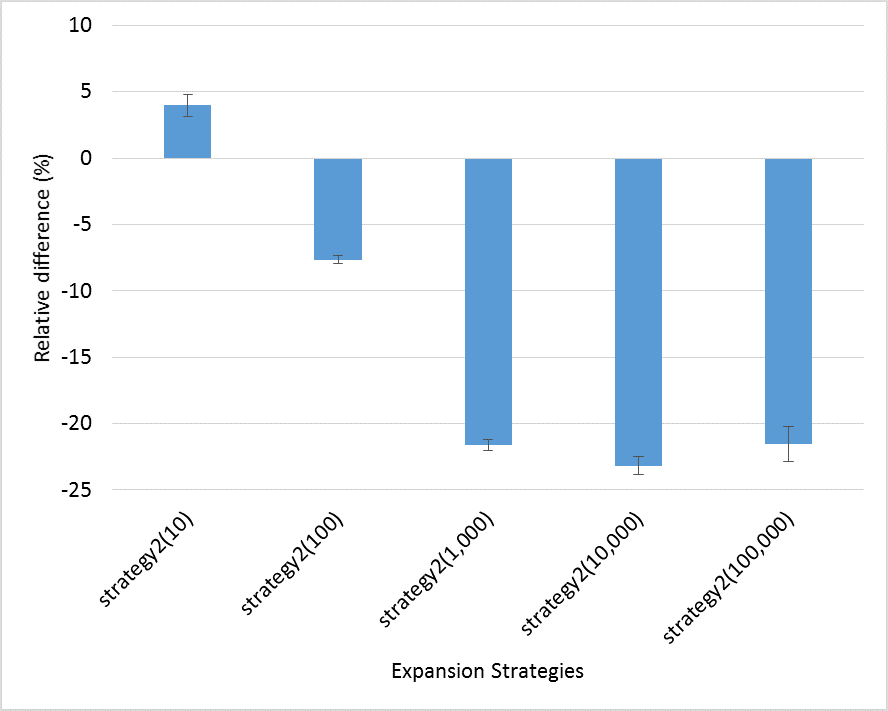
\includegraphics[width=5in]{immagini_extension/breast_strategy2.png}
\caption{Relative gains on Breast Cancer dataset with $minsup$=6, Strategy2 and different $X$ values.
}
\label{breast_strategy2}
\end{figure}

\begin{figure}[!t]
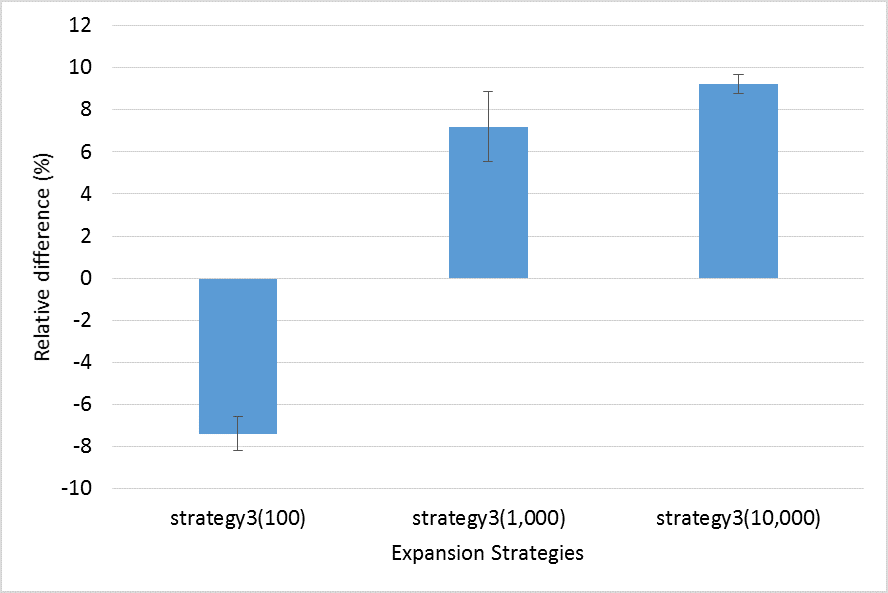
\includegraphics[width=5in]{immagini_extension/breast_strategy3.png}
\caption{Relative gains on Breast Cancer dataset with $minsup$=6, Strategy3 and different $X$ values.
}
\label{breast_strategy3}
\end{figure}

\begin{figure}[!t]
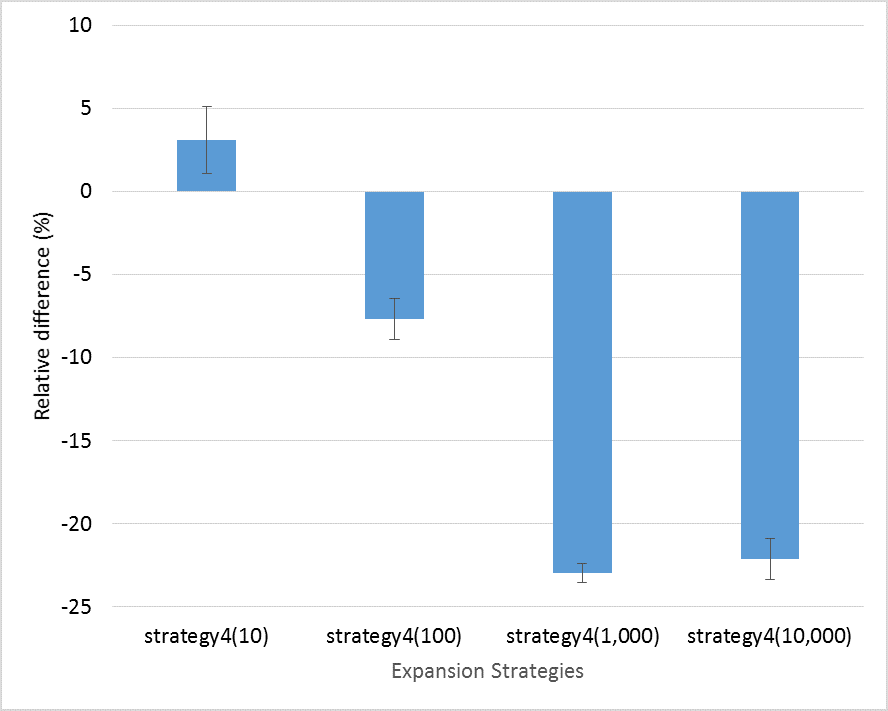
\includegraphics[width=5in]{immagini_extension/breast_strategy4.png}
\caption{Relative gains on Breast Cancer dataset with $minsup$=6, Strategy4 and different $X$ values.
}
\label{breast_strategy4}
\end{figure}

\begin{figure}[!t]
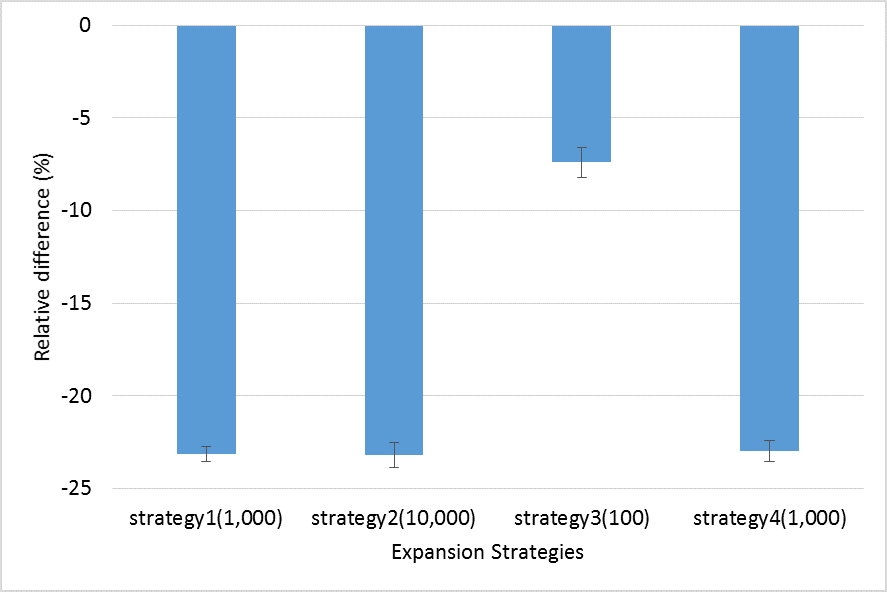
\includegraphics[width=5in]{immagini_extension/breast_strategy_best.png}
\caption{Relative gains of the best configuration for each strategy, on Pems Cancer dataset with $minsup$=6.
}
\label{breast_strategy_best}
\end{figure}

